%
% Unless otherwise indicated, the copyright in this material is 
% owned by Joerg Evermann. This material is licensed to you under the 
% Creative Commons by-attribution non-commercial license (CC BY-NC 4.0)}
%

\section*{Sources and Further Reading}

\begin{tcolorbox}[colback=alert]
Kevin P. Murphy: \emph{Probabilistic Machine Learning -- An Introduction}. MIT Press 2022. \\

\url{https://probml.github.io/pml-book/book1.html} \\

Chapter 15

\end{tcolorbox}

The book by Murphy is freely available and provides three chapters on neural networks, one for structured data, one for images, and one for sequences. It provides significant depth on convolutional and recurrent network architectures, fitting the models, and problems the data analyst may encounter. 

\begin{tcolorbox}[colback=alert]
\subsubsection*{Guides and examples on the Tensorflow and Keras web sites:}

\begin{itemize}
\item \href{https://www.tensorflow.org/tutorials/structured_data/time_series}{Time Series Forecasting (Tensorflow)} \\
\item \href{https://www.tensorflow.org/guide/keras/working_with_rnns}{Working with RNNs (Tensorflow)} \\
\item \href{https://www.tensorflow.org/text/tutorials/text_generation}{Text Generation with an RNN (Tensorflow)} \\
\item \href{https://keras.io/examples/timeseries/timeseries_weather_forecasting/}{Timeseries Forecasting for Weather Prediction (Keras)}
\end{itemize}
\end{tcolorbox}

This course uses the Tensorflow programming framework for neural network applications. The Tensorflow website has a multitude of introductory and advanced guides and tutorial that cover all aspects of machine learning with neural networks. 

\begin{tcolorbox}[colback=alert]
\subsubsection*{Introductory tutorials:}

Olah, Christopher (2015) \href{https://colah.github.io/posts/2015-08-Understanding-LSTMs/}{Understanding LSTM Networks} \\

Karpathy, Andrej (2015) \href{https://karpathy.github.io/2015/05/21/rnn-effectiveness/}{The Unreasonable Effectiveness of Recurrent Neural Networks}
\end{tcolorbox}

Chris Olah has been lead researcher at OpenAI and Google Brain and co-founded Anthropic. Andrej Karpathy has been lead reaserchers at OpenAI and Tesla. Both tutorials are very useful and easy introductions to the topic of recurrent LSTM networks.

\section{Introduction}

Recurrent Neural Networks (RNNs) are a class of neural networks that are used for modeling sequence data such as time series, natural language, or audio. Characterized by their ability to maintain a ''memory'' of previous inputs while processing new ones, RNNs are particularly useful for tasks where historical context is important.

The development of RNNs can be traced back to the 1980s with the introduction of architectures that could use their internal state (memory) to process sequences of inputs. This concept was refined in the 1990s through the introduction of the Long Short-Term Memory (LSTM) network, which significantly improved the performance of RNNs on tasks requiring learning long-term dependencies.

RNNs are employed in a variety of applications, handling different types of data and tasks:
\begin{itemize}
\item \emph{Natural Language Processing (NLP):} RNNs are the basis for many NLP tasks such as machine translation, speech recognition, and text generation. Their ability to process sequences of words and maintain context helps in producing better translations and recognizing speech accurately.
\item \emph{Time Series Prediction:} RNNs are suitable for forecasting future events in financial markets, weather conditions, and other time-dependent phenomena due to their ability to remember past data.
\item \emph{Music and Video Generation:} By learning from sequences of musical notes or frames of videos, RNNs can generate new music pieces and video clips that are similar in style to their training data.
\item \emph{Audio Transcription and Video Captioning:} By examining sequences of audio or visual images, RNNs can generate text transcripts or captions of the video content.  
\item \emph{Healthcare:} In medical diagnostics, RNNs can predict disease progression and patient outcomes by analyzing sequential data such as patient records and time-series observations from medical sensors.
\item \emph{Business Processes:} In business processes, RNNs can be used to predict the next activity, potential problems, time to completion, or other outcomes based on the series of actions already completed.
\end{itemize}

\section{Sequence Models}

Recurrent Neural Networks (RNNs) are called ''recurrent'' because they perform the same task for every element of a sequence, with the output being dependent on the previous computations. RNNs can pass information from one (time or sequence) step of the network to the next. This mechanism is what makes RNNs ''recurrent'' -- they recur or repeat the same process over each part of the input, while maintaining some memory of what has happened before. This memory is maintained through internal or ''hidden'' states of the network, which capture information about earlier elements in the sequence, thereby providing a form of memory. This allows RNNs to process not just individual data points, but entire sequences of data (such as a sentence or a time series), making them effective for tasks where context and order are important.

In using RNNs with sequence data, one can distinguish three types of general model architectures that are useful for different tasks.

\subsubsection*{Seq2Vec}

The sequence-to-vector (''\emph{Seq2Vec}'') model predicts a single outcome or target from a sequence of inputs. This type of model can be a regression or classification model. The general model architecture is shown in Figure~\ref{fig:seqclassification}. The hidden states $h_i$ are connected to model the memory through time. The state of the network depends not only on the current input but also on the previous state, and therefore implicitly on all prior inputs. In practical applications, the inputs, outputs, and hidden state can be high-dimensional vectors or arrays.

\begin{figure}[b]
\centering
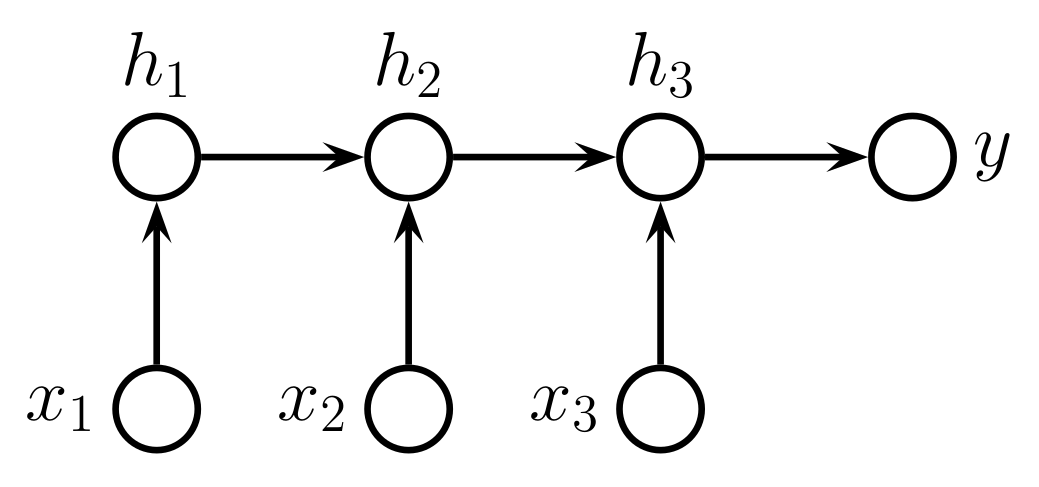
\includegraphics[width=.5\textwidth]{seqclassification} \\

\scriptsize Source: Murphy Fig. 15.4
\caption{Seq2Vec recurrent neural network architecture}
\label{fig:seqclassification}
\end{figure}

This type of architecture is useful for example in sentiment analysis, where it can analyze sequences of text to determine the sentiment expressed, summarizing the overall sentiment in a single vector for classification.

\subsubsection*{Vec2Seq}

The vector-to-sequence (''\emph{Vec2Seq}'') models are designed to generate a sequence from a fixed-length input vector. This approach is commonly used in tasks where a sequence needs to be generated from a compact representation. Figure~\ref{fig:vec2seq} shows an example of such an architecture. A single input $x$ gives rise to multiple outputs $y$ with the hidden states $h$ mainting information about the history. Here, the state of the network depends not only on the single input but also on the previous state and previous output. 

\begin{figure}
\centering
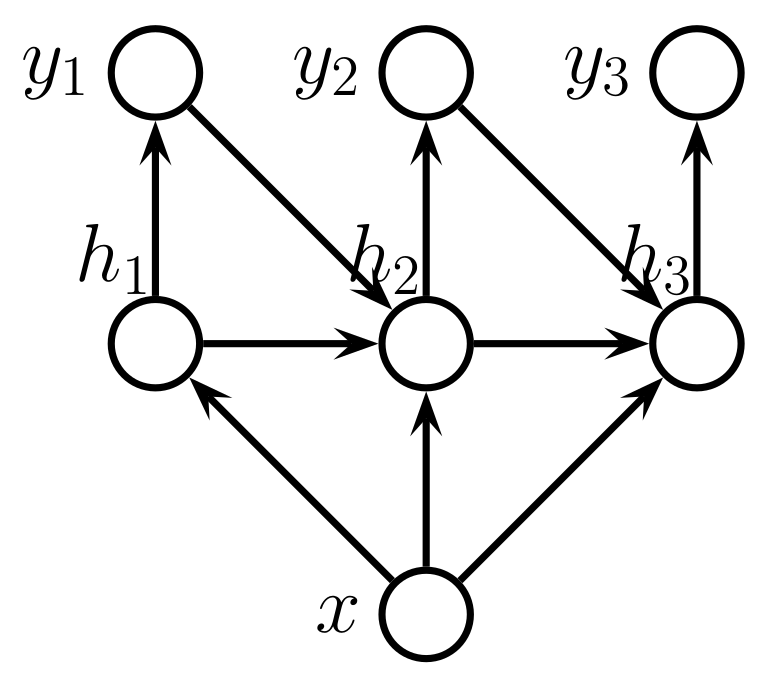
\includegraphics[width=.375\textwidth]{vec2seq.png} \\

\scriptsize Source: Murphy Fig. 15.1
\caption{Vec2Seq recurrent neural network architecture}
\label{fig:vec2seq}
\end{figure}

The Vec2Seq architecture is useful for example in image captioning, generating a sequence of words as descriptive text for a single input image (a vector of pixels). Another use case is music generation, creating a sequence of musical notes from an input vector that encodes a particular style or mood.

\subsubsection*{Seq2Seq}

Sequence-to-sequence (''\emph{Seq2seq}'') models are designed to transform an input sequence into an output sequence. These models are useful for tasks that involve translation or conversion from one sequence to another, maintaining the context from the input to the output. The general architecture is shown in Figure~\ref{fig:seq2seq}. For each input $x$, one output $y$ is generated and the hidden state $h$ maintains information about the history. The state of the network depends not only on the current input, but also on the previous state. Depending on the application, Seq2Seq networks may also employ \emph{bi-directional connections} between hidden layers, as shown in the right panel of Figure~\ref{fig:seq2seq}.

\begin{figure}
\centering
\begin{minipage}{.45\textwidth}
\centering

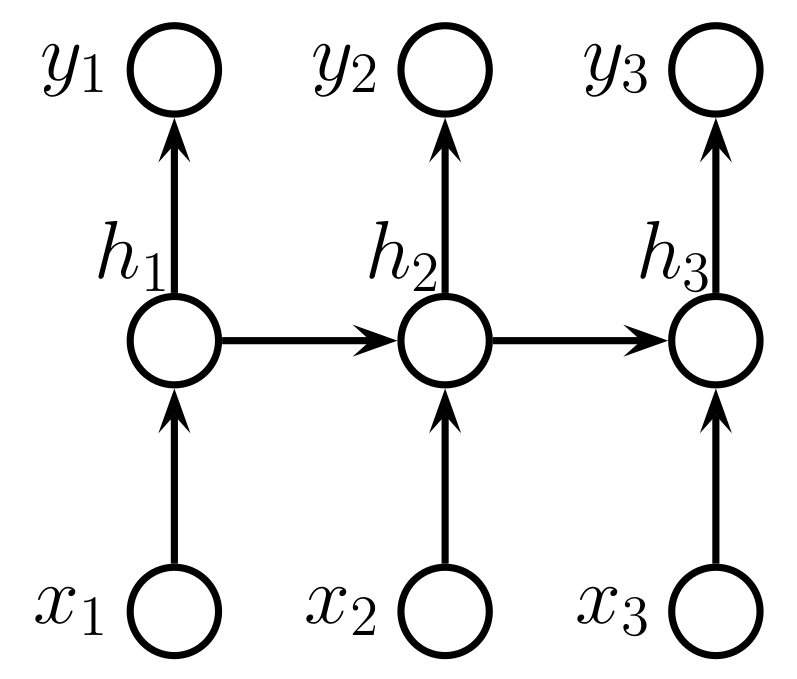
\includegraphics[width=.8\textwidth]{seq2seq.png} 
\end{minipage}
\begin{minipage}{.45\textwidth}
\centering

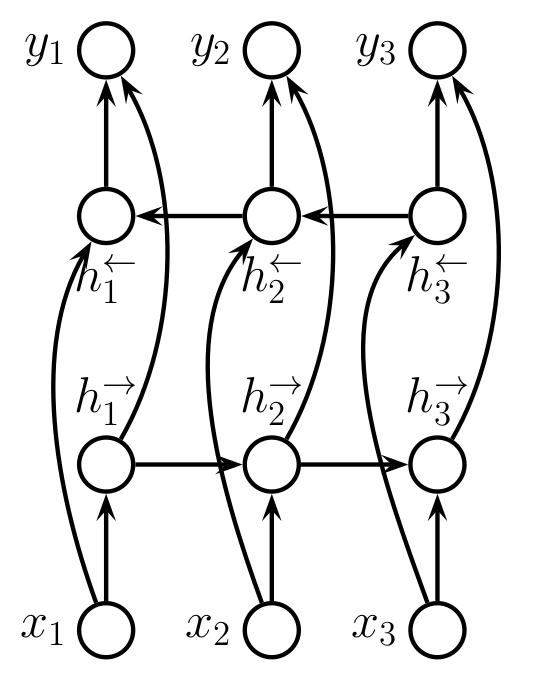
\includegraphics[width=.8\textwidth]{bidiseq2seq.png}
\end{minipage}

\scriptsize Source: Murphy Fig. 15.5
\caption{Seq2Seq recurrent neural network architecture}
\label{fig:seq2seq}
\end{figure}

A typical use case for Seq2Seq models is machine translation from one language to another, where both the input and output are sequences of words. In speech recognition, spoken language is converted into written text, where the audio input is a sequence of phonetic features, and the output is a sequence of words. In video-to-text applications, textual descriptions are generated from video sequences, which involves interpreting sequences of images and producing corresponding sequences of descriptive text.

\section{Unrolling an RNN}

The concept of ''\emph{unfolding}'' or ''\emph{unrolling}'' in recurrent neural networks (RNNs) is a fundamental technique used not only to visualize but more importantly, to implement these networks for sequence processing. Unrolling an RNN refers to the process of expanding the recurrent network through time, transforming it into an equivalent feedforward neural network that represents each time or sequence step explicitly. This helps in understanding and analyzing the behavior of RNNs, especially in training.

An RNN is designed to handle sequences by recursively processing each element of the sequence, maintaining a hidden state that captures information about the past elements of the sequence. When RNN is unrolled, each recurrence becomes a separate, but identical, unit of the network. Each unit corresponds to a time step in the input sequence.

\begin{figure}
\centering
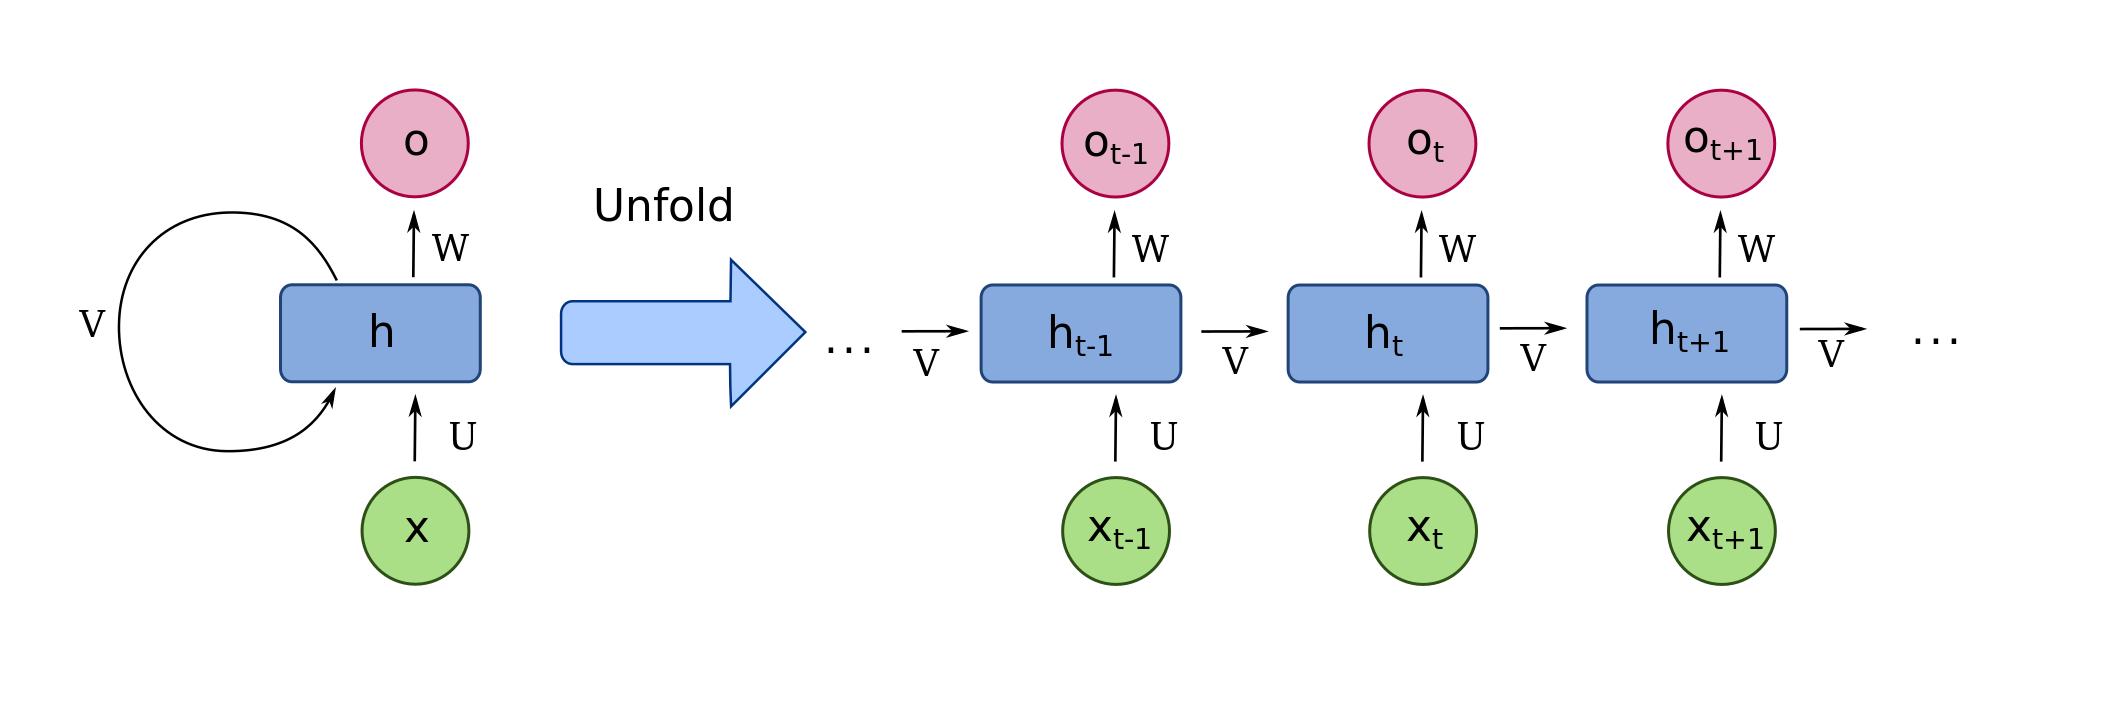
\includegraphics[width=\textwidth]{rnn.png}
\scriptsize \url{https://commons.wikimedia.org/wiki/File:Recurrent_neural_network_unfold.svg}
\caption{Unrolling a recurrent neural network}
\label{fig:unrolling}
\end{figure}

Consider the example in Figure~\ref{fig:unrolling}. The recursive network on the left feeds back information to itself by vector $v$. This information updates the hidden layer's state $h$ from one recurrence (time or sequence step) to the next. This recursive network is unrolled to separate instances of input, hidden layers, and output for each sequence step or time step as shown in the right part of Figure~\ref{fig:unrolling}. The hidden state $h$ and output $o$ in Figure~\ref{fig:unrolling} can be described using basic neural network units:

\begin{align}
h_t &= \sigma ( W_{x} \cdot x_t + W_{h} \cdot h_{t-1} + B_{h}) \label{eq:rnn1} \\
o_t &= \sigma (W_{o} \cdot h_t + B_{o} ) \label{eq:rnn2} 
\end{align}

For example, if the input are sequences of five words and an RNN is designed to process this sequence, unrolling this RNN would result in a chain of five identical neural network units (one for each word). Each unit takes as input the current word, however encoded, and the hidden state output by the previous unit. The first block receives an initial hidden state, often set to zero, which is a starting state.

Unrolling makes the sequence processing capabilities of RNNs explicit and easier to understand, showing how inputs are processed over time. In practice, unrolling an RNN simplifies its implementation, especially for training where gradients are computed across the unfolded network. 

Unrolling an RNN over many time steps can lead to practical challenges. In particular, long unrolled networks with simple units as in Equations~\ref{eq:rnn1} and \ref{eq:rnn2} often suffer from vanishing or exploding gradient problems during training, which makes learning unstable. The vanishing gradient problem in particular means that the network loses its ''memory'' of inputs in the distant past. In other words, such a network is unable to have ''long term'' memory that is useful for many applications.

\section{LSTM Cells}

Long Short-Term Memory (LSTM) cells are a special kind of unit used in recurrent neural networks (RNNs) that are designed to address some of the limitations of traditional RNNs. In particular, they enable networks to learn long-term dependencies that are critical in many sequential tasks such as language modeling or time series prediction. LSTMs were introduced in 1997 as a solution to the vanishing gradient problem commonly encountered in traditional RNNs. Traditional RNNs could perform well on short sequences but struggled with longer ones.

\begin{figure}
\centering

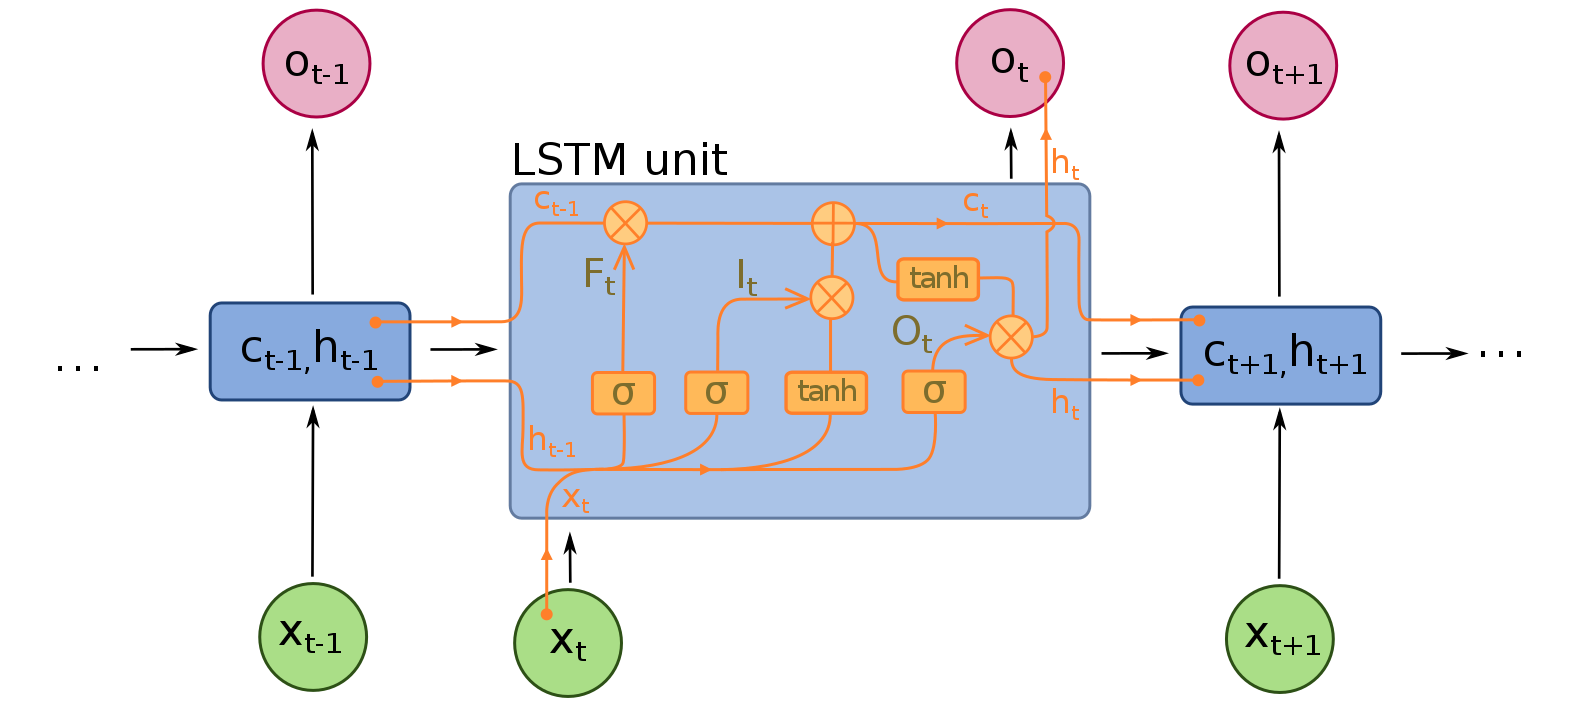
\includegraphics[width=.9\textwidth]{lstm_wikimedia2.png}
\scriptsize \url{https://en.wikipedia.org/wiki/File:Long_Short-Term_Memory.svg} \normalsize
\caption{Long Short-Term Memory Cell}
\label{fig:lstm}
\end{figure}

An LSTM cell, shown schematically in Figure~\ref{fig:lstm}, is complex and contains multiple ''gates'' that regulate the flow of information. LSTM networks have two components to their state. The \emph{cell memory} is represented by $c_t$ and the hidden state is represented by $h_t$ in Figure~\ref{fig:lstm}. Each LSTM cell consists of the following components:

\begin{itemize}
\item \emph{Forget Gate:} This gate decides which information is discarded from the cell memory $c$. It looks at the previous hidden state and the current input and passes its output through a sigmoid function, which outputs numbers between 0 (''forget this vector element completely'') and 1 (''keep this vector element entirely''). The forget gate is represented by $F_t$ in Figure~\ref{fig:lstm} and formally defined as:
\begin{align}
F_t &= \sigma (W_f \cdot [ x_t, h_{t-1}] + b_f) \label{eq:forget}
\end{align}
\item \emph{Input Gate:} This gate updates the cell memory $c$ by adding new information. It looks at the previous hidden state and the current input and includes a sigmoid layer which decides which values to update. It outputs numbers between 0 (''do not update this vector element'') and 1 (''update this vector element completely''). This input gate is represented by $I_t$ in Figure~\ref{fig:lstm} and formally defined as:
\begin{align}
I_t &= \sigma (W_i \cdot [ x_t, h_{t-1}] + b_i) \label{eq:input}
\end{align}
\item \emph{Output Gate:} The output gate examines the prior hidden state and current input. It includes a sigmoid layer which decides which values of the new cell memory to output and pass on to the next cell as the new hidden state. It outputs numbers between 0 (''do not include this vector element in the output'') and 1 (''include this vector element in the output''). The output gate is shown as $O_t$ in Figure~\ref{fig:lstm} and formally defined as:
\begin{align}
O_t &= \sigma (W_o \cdot [ x_t, h_{t-1}] + b_o) \label{eq:output}
\end{align}
\end{itemize}

The outputs of these three gates are used to manipulate the cell memory $c_{t-1}$ that was received from the previous LSTM unit. First, a tanh unit creates a new candidate vector cell memory vector (not explicitly labeled in Figure~\ref{fig:lstm}), formally defined as:
\begin{align}
\tilde{c}_t &= \phi (W_c \cdot [ x_t, h_{t-1}] + b_c) \label{eq:candidate}
\end{align}

The new cell memory $c_t$ is created by first multiplying the old cell memory $c_{t-1}$ with the output of the forget gate $O_t$ (Eq.~\ref{eq:forget}), thus removing some information. Second, information from the candidate cell memory (Eq.~\ref{eq:candidate}) is selected by multiplying it with the values of the input gate $I_t$ (Eq.~\ref{eq:input}) and is then added to the new cell memory. Formally:

\begin{align}
c_t &= F_t \otimes c_{t-1} + I_t \otimes \tilde{c}_t \label{eq:memory}
\end{align}

The output of the LSTM cell is also the new cell state $h_t$. It is formed by applying the output gate $O_t$ (Eq.~\ref{eq:output}) to the cell memory. That is, it selectively outputs and passes on parts of the new cell memory as determined by the output gate. It is formally defined as:

\begin{align}
h_t &= O_t \otimes \phi(c_t) \label{eq:state}
\end{align}

In Equations~\ref{eq:forget} to \ref{eq:state}, $\cdot$ denotes the dot-product (vector product), $\otimes$ denotes element-wise multiplication, and $[.]$ denotes vector concatenation. $\sigma$ is the sigmoid/logistic function and $\phi$ is the hyperbolic tangent (tanh).

\section{GRU Cells}

Gated Recurrent Unit (GRU) cells are a type of recurrent neural network (RNN) architecture introduced as an alternative to Long Short-Term Memory (LSTM) cells. The motivation behind the development of GRUs was to simplify the LSTM architecture, which, although powerful, is also quite complex due to its multiple gates and states. By reducing the number of gates from three to two, GRUs aim to offer a model that can train faster and require fewer computational resources, while still capturing long-range dependencies within the data. GRUs also do not have an internal memory unit separate from the hidden state. While GRUs tend to train faster due to their simpler structure, in some cases LSTMs outperform GRUs in predictive performance, if the additional complexity of LSTMs are appropriate to the data set and task.

\begin{figure}
\centering

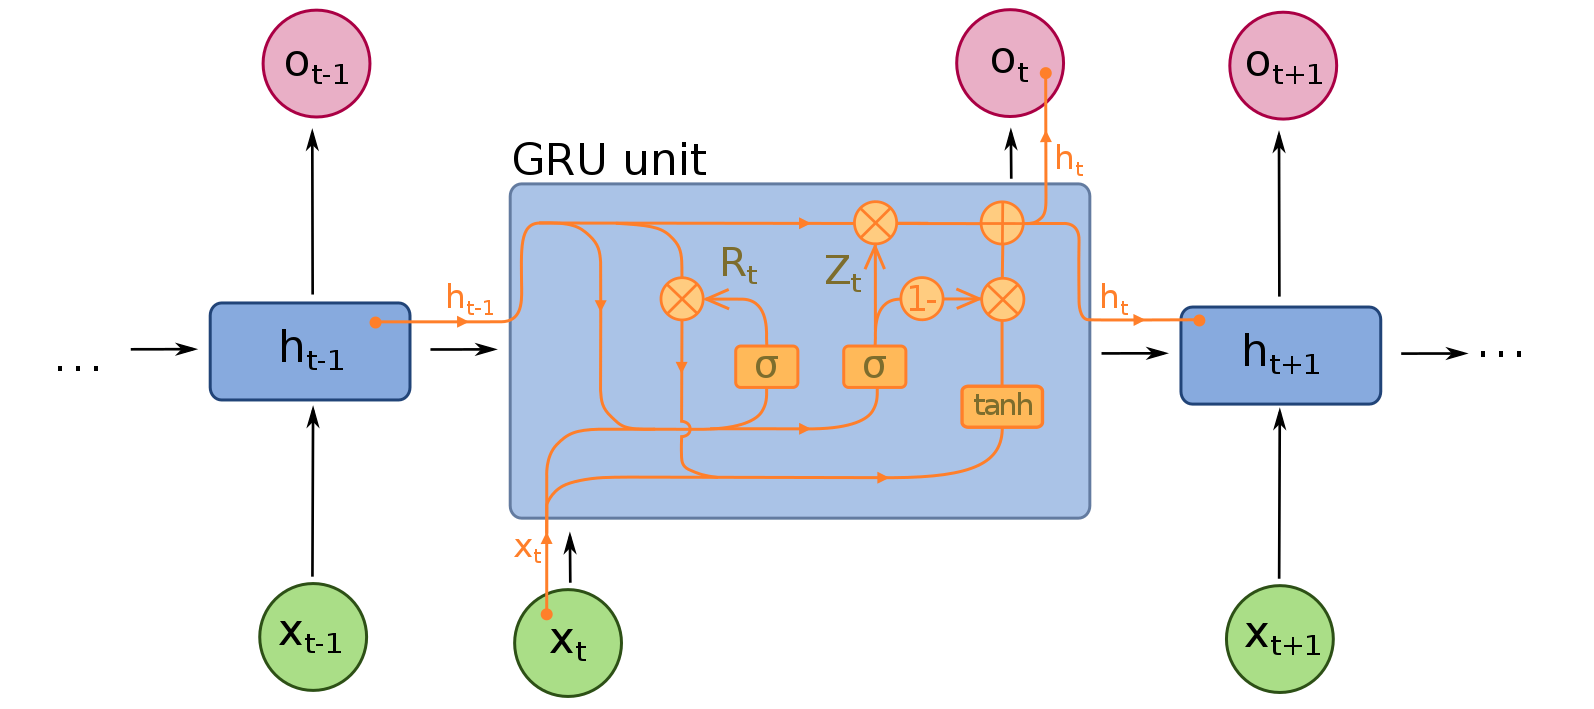
\includegraphics[width=.85\textwidth]{gru_wikimedia.png}
\scriptsize \url{https://en.wikipedia.org/wiki/File:Gated_Recurrent_Unit.svg} \normalsize
\caption{Gated Recurrent Unit (GRU)}
\label{fig:gru}
\end{figure}

A GRU cell, schematically shown in Figure~\ref{fig:gru} consists of only two gates, the \emph{reset gate} and the \emph{update gate}. It also merges the cell memory and the hidden state.

\begin{itemize}
\item \emph{Reset Gate:} This gate, represented as $R_t$ in Figure~\ref{fig:gru}, determines how much past information to forget, which is important for making the model more adaptable to changes in the data sequence. It examines the previous state and current input and applies a sigmoid function. It outputs values between 0 (''reset this vector element completely'') and 1 (''retain this vector element completely'').
\begin{align}
R_t &= \sigma (W_r \cdot [x_t, h_{t-1}] + b_r) \label{eq:reset}
\end{align}
\item \emph{Update Gate:} This gate, represented as $Z_t$ in Figure~\ref{fig:gru}, decides how much of the past information (from previous time or sequence steps) needs to be passed along to the future. It is similar to the combination of the forget and input gates in an LSTM. It examines the previous state and current input, applies a sigmoid function and outputs values between 0 (''do not update this vector element, retain the old state'') and 1 (''update this vector element, discard the old state''). 
\begin{align}
Z_t &= \sigma (W_z \cdot [x_t, h_{t-1}] + b_z) \label{eq:update}
\end{align}
\end{itemize}

The candidate new hidden state is calculated by applying the reset gate to the prior hidden state and then combining the result with the current input and applying a tanh activation function. This ''forgets'' certain information from the prior state. Formally:
\begin{align}
\hat{h}_t &= \phi (W_h \cdot [x_t, R_t \otimes h_{t-1}] + b_h) \label{eq:candidategru}
\end{align}

Finally, the actual new hidden state is calculated as a weighted sum of the past hidden state, weighted by $1-Z_t$, and the candidate state, weighted by $Z_t$.

\begin{align}
h_t &= (1 - Z_t) \otimes h_{t-1} + Z_t \otimes \hat{h}_t \label{eq:gruoutput}
\end{align}

In Equations~\ref{eq:reset} to \ref{eq:gruoutput}, $\cdot$ denotes the dot-product (vector product), $\otimes$ denotes element-wise multiplication, and $[.]$ denotes vector concatenation.  $\sigma$ is the sigmoid/logistic function and $\phi$ is the hyperbolic tangent.

\section{Statefulness}

Recurrent Neural Networks (RNNs) are designed to handle sequence data. One of the key decisions in designing RNNs is whether to use a stateful or stateless configuration. This choice affects how the network processes sequences and learns from data, influencing both the training process and application effectiveness.

In \emph{stateless RNNs}, the internal state is reset for each batch of training data. This means that the learning and predictions are independent of the previous batch. The network starts with a clean slate for every input sequence, making no assumptions based on past data points within the same batch. Since stateless RNNs treat each input sequence as independent, training can be simpler and faster. There is no need to maintain and manage state continuity across batches, and batches can be assembled from the input sequences in arbitrary order and randomly shuffled. Stateless RNNs are typically used when sequences are short enough to fit within the number of unrolled RNN steps and the context within a single sequence is sufficient for the prediction task.

\emph{Stateful RNNs} maintain the internal state between batches, allowing the network to retain information across different input batches. This is useful when sequences are longer than the number of unrolled steps. Training stateful RNNs requires careful management of the state so that it is carried over appropriately across batches. Batches cannot be randomly drawn and cannot be shuffled. The state must be reset manually at the start of each epoch or when starting a new sequence. Stateful RNNs are advantageous for tasks involving long sequences where the context needs to be maintained over long periods, such as in time-series analysis or long-form text processing.

\section{Example -- Stock Market Prediction}

This example uses historic stock market data to predict future performance. In particular, it uses data for the Dow Jones Industrial Average (DJIA) that was exported from the \texttt{quarks} library for R. The data set encompasses opening closing, low, and high values, as well as trading volume for every day between the years 2000 and 2021 (converted to Euros). This is a regression problem with the targets being the difference in closing prices to the next day.

\begin{tcolorbox}[colback=code]
\footnotesize
Complete implementations for this and the other examples in this chapter are available in the following GitHub repo:
\url{https://github.com/jevermann/busi4720-ml} \\

The project can be cloned from this URL: \url{https://github.com/jevermann/busi4720-ml.git}
\normalsize
\end{tcolorbox}

First, load all required packages, specify parameters for the network architecture and training, and then read the data file:

\begin{samepage}
\begin{pythoncode}
import math
import tensorflow as tf
from tensorflow import keras
from keras import layers
import pandas as pd

tf.random.set_seed(123)   # Set random seed
n_steps = 20              # Unfold for 20 steps
n_epochs = 25             # Train for 25 epochs

# The read the data set
data = pd.read_csv('https://evermann.ca/busi4720/djia.data.csv')
\end{pythoncode}
\end{samepage}

In the next step, additional features are created. In time series analysis it is often useful to examine the differences between successive values and the relative or percentage changes. The following Python code fragmeent adds these to the data set by applying the Pandas functions \texttt{diff()} and \texttt{pct\_change()} tn the columns of the data frame and concatenating the differences and percentage changes to the dataframe by column.

\begin{samepage}
\begin{pythoncode}
data = pd.concat([data,
    data.diff().add_suffix('diff'),
    data.pct_change().add_suffix('pct')],
    axis=1).iloc[1:,]
\end{pythoncode}
\end{samepage}

When splitting the data into training and validation set, random shuffling cannot be used because the data set is time series data. In other words, information from future observations should not be used in the training set to help predict values of past observations. The following Python code uses the first $80\%$ of the data set for training and the remainder for validation:

\begin{samepage}
\begin{pythoncode}    
# Split data, no random shuffling for time series
train = data[:math.floor(0.8*data.shape[0])]
valid = data.drop(train.index)
\end{pythoncode}
\end{samepage}

Normalizing the data to zero means and unit standard deviation must again only use information from the training data set, even if that means the actual validation set standard deviations are not exactly equal to 1:

\begin{samepage}
\begin{pythoncode}
# Normalize data using only info from training set.
train_mean = train.mean()
train_sd = train.std()
train = (train - train_mean)/train_sd
valid = (valid - train_mean)/train_sd
\end{pythoncode}
\end{samepage}

An easy way to create appropriate sequence batches and targets is to use the Keras function \texttt{timeseries\_dataset\_from\_array()}. It accepts the features, the targetsm and arguments about the sequence length, batch size, and whether the data should be shuffled between batches. This first example will use a stateless LSTM so that the input can be shuffled. This is a regression problem with the target being the closing price difference to the following day.

\begin{samepage}
\begin{pythoncode}
dataset_train = keras.preprocessing.timeseries_dataset_from_array(
    train.drop('price.closediff', axis=1), train['price.closediff'],
    sequence_length=n_steps,
    batch_size=32,
    shuffle=True)

dataset_valid = keras.preprocessing.timeseries_dataset_from_array(
    valid.drop('price.closediff', axis=1), valid['price.closediff'],
    sequence_length=n_steps,
    batch_size=32,
    shuffle=True)
\end{pythoncode}
\end{samepage}

\subsection*{Tensorflow Datasets for Sequence Data}

To see how Tensorflow manages time series or sequence data in its datasets, it is instructive to work with a simple example. Consider the following Pandas dataframe of inputs and targets:

\begin{samepage}
\begin{pythoncode}
test = pd.DataFrame([[0, 0], [1, 1], [2, 2,], [3, 3], 
                     [4, 4], [5, 5], [6, 6], [7, 7]]) 
inputs = test.iloc[:-1,0]
targets = test.iloc[2:,1]

pd.DataFrame([inputs, targets])
\end{pythoncode}
\end{samepage}

\begin{samepage}
\begin{textcode}
     0    1    2    3    4    5    6    7
0  0.0  1.0  2.0  3.0  4.0  5.0  6.0  NaN
1  NaN  NaN  2.0  3.0  4.0  5.0  6.0  7.0
\end{textcode}
\end{samepage}

The first example illustrates creating a dataset object that provides batches of size 2 for a sequence length of 2, using a stride of 1 across the input sequences. This example does not shuffle the data between batches and is therefore suitable for stateful RNNs:

\begin{samepage}
\begin{pythoncode}
ds = keras.preprocessing.timeseries_dataset_from_array(
     inputs, targets,
     batch_size=2, sequence_length=2, sequence_stride=1, shuffle=False)
for element in ds.as_numpy_iterator():
     print(element)
\end{pythoncode}
\end{samepage}

The following output shows batches of sequences and their targets. Note how the sequences are continuous across batchs. For example the first sequence of 2 elements of the first batch is $[0, 1]$ and the first sequence of 2 elements of the second batch is $[2, 3]$, that is, the second batch continues sequences from the first batch, and the hidden state in the LSTM or GRU cells in the RNN can be carried over to the next batch. 
 
\begin{samepage}
\begin{textcode}
(array([[0, 1],
       [1, 2]]), array([2, 3]))
(array([[2, 3],
       [3, 4]]), array([4, 5]))
(array([[4, 5],
       [5, 6]]), array([6, 7]))
\end{textcode}
\end{samepage}

In contrast, the next example shuffles elements between batches and is suitable for stateless RNNs where state is not maintained between batches:

\begin{samepage}
\begin{pythoncode}
ds = keras.preprocessing.timeseries_dataset_from_array(
     inputs, targets, 
     batch_size=2, sequence_length=2, sequence_stride=1, shuffle=True)
for element in ds.as_numpy_iterator():
     print(element)
\end{pythoncode}
\end{samepage}

The output below clearly shows the differences. The sequences of length 2 are not continuous across batches. For example, the first sequence of 2 elements in the second batch is $[5, 6]$ while the first sequence of 2 elements in the third batch is $[3, 4]$.

\begin{samepage}
\begin{textcode}
(array([[4, 5],
       [2, 3]]), array([6, 4]))
(array([[5, 6],
       [0, 1]]), array([7, 2]))
(array([[3, 4],
       [1, 2]]), array([5, 3]))
\end{textcode}
\end{samepage}

The next example shows the effect of varying the sequence stride and the batch size. The batch size is now set to 1, and the sequence stride is 2, that is, after assembling a series of 2 elements for a batch, the next set of 2 elements is taken from two positions further in the input.

\begin{samepage}
\begin{pythoncode}
ds = keras.preprocessing.timeseries_dataset_from_array(
     inputs, targets,
     batch_size=1, sequence_length=2, sequence_stride=2, shuffle=False)
for element in ds.as_numpy_iterator():
     print(element)
\end{pythoncode}
\end{samepage}

\begin{samepage}
\begin{textcode}
(array([[0, 1]]), array([2]))
(array([[2, 3]]), array([4]))
(array([[4, 5]]), array([6]))
\end{textcode}
\end{samepage}

In this small illustrative example, every step of the feature sequence is a single number, whereas in the stock market prediction example every step of the feature sequence is itself a vector of values.


\begin{tcolorbox}[colback=code]
\subsubsection*{Hands-On Exercise} 
Using the simple example data from above to:
\begin{enumerate}
   \item Experiment with different values for \texttt{batch\_size},
   \item Experiment with different values for \texttt{sequence\_length},
   \item Experiment with different values for \texttt{sequence\_stride}.
\end{enumerate}
\end{tcolorbox}

The stock market prediction example uses a sequential neural network model with an input layer to specify the shape of the features to be used for training, one LSTM layer and a dense (fully-connected) layer with a single output for regression. It has the following characteristics:

\begin{itemize}
   \item Hidden state and cell memory size: \texttt{units=16}
   \item ''Seq2Vec'' model: \texttt{return\_sequences=False}
   \item Stateless model: \texttt{stateful=False}
\end{itemize}

Note that the second dimension of the input shape is one less than the total number of columns in the training data, because the column of target values has been removed.

\begin{samepage}
\begin{pythoncode}
model = keras.Sequential()
model.add(layers.InputLayer(
    input_shape=(n_steps, len(train.columns)-1)))
model.add(layers.LSTM(
    units=16,
    return_sequences=False,
    return_state=False,
    stateful=False))
model.add(layers.Dense(1))
model.summary()
\end{pythoncode}
\end{samepage}

The model summary is shown below. It is instructive to verify the number of parameters. Weights and biases are shared between time steps; recall that the RNN actually has a single LSTM cell and unrolling is simply there to make the computation easier. That is, the total parameter count reported below is for a single LSTM cell. Equations~\ref{eq:forget} to \ref{eq:candidate} show that the forget, input and output gates as well as the candidate new memory of the LSTM unit use the same number of parameters, that is, each equation introduces $1984/4 = 496$ parameters. The Equations~\ref{eq:forget} to \ref{eq:candidate} operate on the concatenation of the hidden state and the input, that is on a vector of $16 + 14 = 30$ units. Each equation adds a bias term. Hence, the total number of weights and bias for each gate as $(16 + 14 + 1) * 16 = 496$.

\begin{samepage}
\begin{textcode}
Model: "sequential_4"
_________________________________________________________________
 Layer (type)                Output Shape              Param #   
=================================================================
 lstm_1 (LSTM)               (None, 16)                1984      
 dense_8 (Dense)             (None, 1)                 17        
=================================================================
Total params: 2001 (7.82 KB)
Trainable params: 2001 (7.82 KB)
Non-trainable params: 0 (0.00 Byte)
\end{textcode}
\end{samepage}

Compile and fit the model:
\begin{samepage}
\begin{pythoncode}
model.compile(loss='mean_squared_error', optimizer='Adagrad')

model.fit(dataset_train, epochs=n_epochs,
          validation_data=dataset_valid)
\end{pythoncode}
\end{samepage}
The training output, shown below, indicates that the training loss after 25 epochs is $\approx 1.00$ and the validation is $\approx 7.06$. Importantly, neither training nor validation loss have decreased during training, suggesting that either the neural network model is inappropriate or the problem of stock market prediction is quite difficult.

\begin{textcode}
Epoch 1/25
138/138 [==============================] - 2s 6ms/step -
 loss: 1.0933 - val_loss: 7.0730

Epoch 25/25
138/138 [==============================] - 1s 5ms/step -
 loss: 1.0028 - val_loss: 7.0621
\end{textcode}

\begin{tcolorbox}[colback=code]
\subsubsection*{Hands-On Exercise} 

Download the Python code from \href{https://raw.githubusercontent.com/jevermann/busi4720-ml/main/lstm_example.py}{here}. Then:

\begin{enumerate}
   \item Predict the percentage change of the closing value (column \texttt{price.closepct})
   \item Predict the actual closing value (column \texttt{price.close})
   \item Comment on the model performance results. Are these values more or less predictable than the differenced closing values?
\end{enumerate} \vspace{\baselineskip}

Experiment with different model characteristics:
\begin{enumerate}
    \item Vary the size of the LSTM hidden state and output (\texttt{unit=16}).
    \item Swap the LSTM layer for a GRU layer (\texttt{layers.GRU}). The Keras GRU layer construction function takes the same arguments as the Keras LSTM layer construction function.
    \item Comment on the model performance results.
\end{enumerate}
\end{tcolorbox}

Given the poor performance of the single layer LSTM network, it is natural to ask whether more LSTM layers can make a difference. To illustrate the use of Seq2Seq models, the following model stacks two LSTM layers. Note that the first LSTM layer is a Seq2Seq type that returns an output for each step of the sequence. These outputs form the inputs for the second LSTM layer. That second layer is a Seq2Vec model that returns a single output. The model also adds a second fully-connected layer and droput layers to prevent overfitting. 

\begin{samepage}
\begin{pythoncode}
model = keras.Sequential()
model.add(layers.InputLayer(
    input_shape=(n_steps, len(train.columns)-1)))
model.add(layers.LSTM(
    units=16, return_sequences=True, stateful=False))
model.add(layers.Dropout(rate=0.25))
model.add(layers.LSTM(
    units=16, return_sequences=False, stateful=False))
model.add(layers.Dense(32))
model.add(layers.Dropout(rate=0.25))
model.add(layers.Dense(1))
model.summary()
\end{pythoncode}
\end{samepage}

The model summary and the final epoch training output are shown below. Unfortunately, the model performs no better than the simple one.

\begin{samepage}
\begin{textcode}
_________________________________________________________________
 Layer (type)                Output Shape              Param #   
=================================================================
 lstm_2 (LSTM)               (None, 20, 16)            1984      
 dropout_3 (Dropout)         (None, 20, 16)            0         
 lstm_3 (LSTM)               (None, 16)                2112      
 dense_9 (Dense)             (None, 32)                544       
 dropout_4 (Dropout)         (None, 32)                0         
 dense_10 (Dense)            (None, 1)                 33        
=================================================================
Total params: 4673 (18.25 KB)
Trainable params: 4673 (18.25 KB)
Non-trainable params: 0 (0.00 Byte)

Epoch 25/25
138/138 [==============================] - 2s 17ms/step 
- loss: 1.0064 - val_loss: 7.1526
\end{textcode}
\end{samepage}

Perhaps more history than the last 20 steps is required for good predictions. The following example illustrates a stateful LSTM. First, change the batch size to 1 for a single sequence of continuous elements and prohibit shuffling of the data set:

\begin{samepage}
\begin{pythoncode}
dataset_train = keras.preprocessing \
    .timeseries_dataset_from_array(
    train.drop('price.closediff', axis=1),
    train['price.closediff'],
    sequence_length=n_steps,
    sampling_rate=1, batch_size=1, shuffle=False)

dataset_valid = keras.preprocessing \
    .timeseries_dataset_from_array(
    valid.drop('price.closediff', axis=1),
    valid['price.closediff'],
    sequence_length=n_steps,
    sampling_rate=1, batch_size=1, shuffle=False)
\end{pythoncode}
\end{samepage}

The neural network architecture is a single LSTM as in the initial example, but this time the LSTM layer is stateful. Note that the input layer does not specify a sequence length for the batch input shape.

\begin{samepage}
\begin{pythoncode}
model = keras.Sequential()
model.add(layers.InputLayer(
    batch_input_shape=(1, None, len(train.columns)-1)))
model.add(layers.LSTM(units=16,
    return_sequences=False, return_state=False, stateful=True))
model.add(layers.Dense(1))
model.summary()
\end{pythoncode}
\end{samepage}

Again, this model does not perform any better than the previous two models. As a baseline comparison, a Vec2Vec model is fitted with a single large feature vector that contains all 20 sequence steps. A \texttt{Flatten} layer is used to re-shape the inputs from shape $[None, 20, 14]$ to $[None, 280]$ where the first index is the batch size which is flexible and depends on how the data set is prepared.

\begin{samepage}
\begin{pythoncode}
model = keras.Sequential()
model.add(layers.InputLayer(
    input_shape=(n_steps, len(train.columns)-1)))
model.add(layers.Flatten())
model.add(layers.Dense(256))
model.add(layers.Dropout(rate=0.25))
model.add(layers.Dense(64))
model.add(layers.Dropout(rate=0.25))
model.add(layers.Dense(1))
model.summary()
\end{pythoncode}
\end{samepage}

It turns out this model performs significantly better than any of the three previous LSTM models. However, the model summary indicates a very large number of model parameters, almost 50 times the number of the basic LSTM model, making this model much more flexible and powerful than the earlier LSTM models:

\begin{samepage}
\begin{textcode}
Model: "sequential"
_________________________________________________________________
 Layer (type)                Output Shape              Param #   
=================================================================
 flatten (Flatten)           (None, 280)               0         
 dense (Dense)               (None, 256)               71936     
 dropout (Dropout)           (None, 256)               0         
 dense_1 (Dense)             (None, 64)                16448     
 dropout_1 (Dropout)         (None, 64)                0         
 dense_2 (Dense)             (None, 1)                 65        
=================================================================
Total params: 88449 (345.50 KB)
Trainable params: 88449 (345.50 KB)
Non-trainable params: 0 (0.00 Byte)
\end{textcode}
\end{samepage}

\section{Next Activity Prediction in Business Processes}

As another example of a sequence data problem, consider predicting the next activity in a running instance of a business process. In particular, train a model to predict the next activity from a prefix sequence of 5 activities that have already occurred. This is a classification problem, where the class of the next activity is to be predicted. 

\begin{tcolorbox}[colback=code]
\footnotesize
Complete implementations for this and the other examples in this chapter are available in the following GitHub repo: \url{https://github.com/jevermann/busi4720-ml} \\

The project can be cloned from this URL: \url{https://github.com/jevermann/busi4720-ml.git}

Download the example event log here\footnote{
The example log file is taken from the \href{
https://doi.org/10.4121/uuid:3926db30-f712-4394-aebc-75976070e91f}{4TU repository} where it has been published under the \href{ https://data.4tu.nl/articles/_/12721292/1}{4TU general terms of use}.
}: \url{https://evermann.ca/busi4720/BPI_Challenge_2012.xes.gz}
\normalsize
\end{tcolorbox}

First, import the required libraries and use PM4Py to read the event log:

\begin{samepage}
\begin{pythoncode}
import numpy
from tensorflow import keras
from keras import layers
import pandas as pd
import pm4py

# Length of sequences to predict from
prefix_len= 5   

# Read the log
log = pm4py.read_xes('BPI_Challenge_2012.xes.gz')  
\end{pythoncode}
\end{samepage}

Preprocess the data by fixing data types after the import and filtering the log for activity completion events:

\begin{samepage}
\begin{pythoncode}
log['time:timestamp'] = pd.to_datetime(log['time:timestamp'],utc=True)
log['case:REG_DATE'] = pd.to_datetime(log['case:REG_DATE'],utc=True)
log['case:AMOUNT_REQ'] = pd.to_numeric(log['case:AMOUNT_REQ'])
log['org:resource'] = log['org:resource'].astype(str)

# Retain only activity completion events
log = log[log['lifecycle:transition'] == 'COMPLETE']
\end{pythoncode}
\end{samepage}

Filter and sort the log for cases that contain 6 or more activities (5 to predict from, plus one target):

\begin{samepage}
\begin{pythoncode}
# Find the case start time as time of the first event in case
log = log.merge(log.groupby('case:concept:name',as_index=False) \
    ['time:timestamp'].min() \
    .rename(columns={'time:timestamp':'case:start'}), how='left')
    
# Find the number of events for each case
log = log.merge(log.groupby('case:concept:name', as_index=False) \
    ['time:timestamp'].count(). \
    rename(columns={'time:timestamp':'num_events'}), how='left')
    
# Filter log for minimum 6 events (5 input, 1 target)
log = log[log['num_events'] > prefix_len]
# Sort log by case start, then by event time
log.sort_values(['case:start', 'time:timestamp'], inplace=True)
\end{pythoncode}
\end{samepage}

Next, specify the feature column:

\begin{pythoncode}
# This is the feature to predict (from)
f_name = 'concept:name'
\end{pythoncode}

Next, identify the ''vocabulary'', that is, the set of unique activity names for inputs and targets. Rather than converting this to integers using a Keras preprocessing layer, the following code block builds dictionary objects for converting activity names to and from integers. Note that a special end-of-case marker is added to the set of activity names.

\begin{samepage}
\begin{pythoncode}
# Vocabulary
vocab = list(log[f_name].unique()) + ['EOC']
v_size = len(vocab)

# Dictionaries to convert to/from integers
f2int = dict([(s, vocab.index(s)) for s in vocab])
int2f = dict([(v, k) for (k, v) in f2int.items()])
\end{pythoncode}
\end{samepage}

The following code block creates a list of activity for each case. This is done by grouping the data frame by case ID (''\texttt{case:concept:name}'') and then using the \texttt{apply(list)} function to the feature columns of the grouped data frame and naming the resulting column \texttt{features}:

\begin{samepage}
\begin{pythoncode}
# Make sequences of feature names for each case
features = log.groupby(['case:concept:name'])[f_name] \
    .apply(list).reset_index(name='features')
\end{pythoncode}
\end{samepage}

The end-of-case marker is added to each list just created and the lists are then converted to lists of integers using the dictionary built earlier:

\begin{samepage}
\begin{pythoncode}
sequences=[l+['EOC'] for l in list(features['features'])]
sequences=[[f2int[i] for i in seq] for seq in sequences]
\end{pythoncode}
\end{samepage}

Split sequences into prefix and target using a sliding window over each sequence:
\begin{samepage}
\begin{pythoncode}
data = pd.DataFrame([(seq[i:i+prefix_len], \
    seq[i+prefix_len]) for seq in sequences \
    for i in range(len(seq)-prefix_len)])
\end{pythoncode}
\end{samepage}

Then, split the sequence elements into their own data frame columns, that is Pandas Series:

\begin{samepage}
\begin{pythoncode}
# Split the lists into dataframe columns
data = data.assign(**data[0].apply(pd.Series).add_prefix('index_'))
\end{pythoncode}
\end{samepage}

Treating each prefix as independent, split the data randomly into a training and validation set. 

\begin{samepage}
\begin{pythoncode}
# Divide into train and test set
train = data.sample(frac=0.8)
valid = data.drop(train.index)
\end{pythoncode}
\end{samepage}

Then, separate the features from the targets:

\begin{samepage}
\begin{pythoncode}
# Separate X and Y
train_x = train.iloc[:,2:]
train_y = train.iloc[:,1]
valid_x = valid.iloc[:,2:]
valid_y = valid.iloc[:,1]
\end{pythoncode}
\end{samepage}

The neural network model is a single-layer stateless LSTM with a Seq2Vec architecture. The input layer specifies the input shape as 5 sequence steps with an undetermined feature size. The features, that is, the activity numbers, are passed to a word embedding layer with 16 output dimensions. That is, each activity number is transformed into a set of 16 values. Note that this occurs for each of the 5 sequence steps fed into the network. Each embedding output is then provided as the input feature vector to the LSTM layer. The LSTM output is passed to a fully-connected output layer with as many units as there are different activity names. The activation function is a softmax function so that this layer returns class membership probabilities. 

\begin{samepage}
\begin{pythoncode}
model = keras.Sequential()
model.add(layers.InputLayer(input_shape=(5,)))
model.add(layers.Embedding(input_dim=v_size, output_dim=16))
model.add(layers.LSTM(units=32,
    return_sequences=False, return_state=False, stateful=False))
model.add(layers.Dense(v_size, activation='softmax'))
\end{pythoncode}
\end{samepage}

Finally, the model is compiled and trained for 25 epochs:

\begin{samepage}
\begin{pythoncode}
# Compile with loss and optimizer
model.compile(loss='sparse_categorical_crossentropy',
              optimizer='Adagrad',
              metrics=['sparse_categorical_accuracy'])

# Train the model and validate on
model.fit(train_x, train_y,
          validation_data=(valid_x, valid_y),
          epochs=25, shuffle=True)
\end{pythoncode}
\end{samepage}

The model summary is shown below, as well as the training progress information for the first and last epoch. The prediction accuracy improves significantly from the first epoch, for both the training and the validation dataset. Additionally, the training and validation losses are similar, suggesting the model does not overfit.

\begin{samepage}
\begin{textcode}
_________________________________________________________________
 Layer (type)                Output Shape              Param #   
=================================================================
 embedding (Embedding)       (None, 5, 16)             384       
 lstm (LSTM)                 (None, 32)                6272      
 dense (Dense)               (None, 24)                792       
=================================================================
Total params: 7448 (29.09 KB)
Trainable params: 7448 (29.09 KB)
Non-trainable params: 0 (0.00 Byte)

Epoch 1/25
2875/2875 [==============================] - 7s 2ms/step - 
loss: 3.0962 - sparse_categorical_accuracy: 0.1984 - 
val_loss: 3.0310 - val_sparse_categorical_accuracy: 0.2013

Epoch 25/25
2875/2875 [==============================] - 6s 2ms/step - 
loss: 1.4728 - sparse_categorical_accuracy: 0.5886 - 
val_loss: 1.4553 - val_sparse_categorical_accuracy: 0.5935
\end{textcode}
\end{samepage}

To predict from the trained model, use the Keras \texttt{predict()} function of the fitted model. The following Python code block takes as input a sequence from the training data set, and predicts the class membership probabilities, that is the probabilities over the following process activity. The predicted activity is determined by sampling from the class membership. Alternatively, the most likely class could be chosen. Both options can be combined in that a random choice is made between sampling from the probabilites and choosing the most likely class. 

\begin{samepage}
\begin{pythoncode}
input = train_x.iloc[2:3,:].copy()
print(input)

# Take the probabilities of the first entry of the return batch
probs = model.predict(input)[0]

# Either deterministically choose the most probable class
# pred = probs.argmax()
# Better is to randomly sample from the probabilities
pred = numpy.random.choice(a=range(v_size), p=probs)

# Print the result
print(int2f[pred])
\end{pythoncode}
\end{samepage}

The chosen activity is added to the end of the input sequence and the prediction is repeated until the end of the case is predicted.

\begin{samepage}
\begin{pythoncode}
# And keep doing this until end-of-case is reached
while int2f[pred] != 'EOC':
    for i in range(4):
        input.iat[0,i] = input.iat[0, i+1]
    input.iat[0,4] = pred
    print(input)
    probs = model.predict(input)[0]
    pred = numpy.random.choice(a=range(v_size),p=probs)
    print(int2f[pred])
\end{pythoncode}
\end{samepage}

An example output is shown below. The exact result depends on the specific parameter values of the trained model and the sampling of the class probabilities.

\begin{samepage}
\begin{textcode}
      index_0  index_1  index_2  index_3  index_4
4380        9       10        9       15       13
1/1 [==============================] - 0s 11ms/step
W_Nabellen incomplete dossiers
      index_0  index_1  index_2  index_3  index_4
4380       10        9       15       13       21
1/1 [==============================] - 0s 13ms/step
O_ACCEPTED
      index_0  index_1  index_2  index_3  index_4
4380        9       15       13       21       13
1/1 [==============================] - 0s 12ms/step
W_Nabellen offertes
      index_0  index_1  index_2  index_3  index_4
4380       15       13       21       13        9
1/1 [==============================] - 0s 13ms/step
W_Valideren aanvraag
      index_0  index_1  index_2  index_3  index_4
4380       13       21       13        9       15
1/1 [==============================] - 0s 16ms/step
EOC
\end{textcode}
\end{samepage}

%\begin{frame}[fragile]{Next Activity Prediction of a Business Process \small [cont'd]}
%Alternative model with stacked and bi-directional LSTM:
%\begin{pythoncode}
%model = keras.Sequential()
%model.add(layers.InputLayer(input_shape=(5,)))
%model.add(layers.Embedding(input_dim=v_size,
                           %output_dim=16))
%model.add(
    %layers.Bidirectional(
        %layers.LSTM(units=32,
                    %return_sequences=True,
                    %return_state=False,
                    %stateful=False)))
%model.add(
    %layers.LSTM(units=32,
                %return_sequences=False,
                %return_state=False,
                %stateful=False))
%model.add(layers.Dense(v_size, activation='softmax'))
%\end{pythoncode}
%\end{frame}

\begin{tcolorbox}[colback=code]
\subsubsection*{Hands-On Exercise} 

Download the \href{https://github.com/jevermann/busi4720-ml/blob/main/process_prediction.py}{complete Python file} and the \href{https://evermann.ca/busi4720/BPI_Challenge_2012.xes.gz}{example event log}. \\

Adapt the network architecture to identify the impact on training and validation performance of the following:
   \begin{enumerate}
      \item Dropouts in the LSTM layer (use the \texttt{dropout} option when defining the LSTM layer)
      \item GRU instead of LSTM layers (use \texttt{layers.GRU()})
      \item Embedding size (originally 16, note: vocabulary size is 23+1)
      \item Further training epochs (originally 25)
   \end{enumerate}
Comment on your findings and identify the best model. \\
\end{tcolorbox}

\section{Review Questions}
\paragraph*{Introduction}
\begin{enumerate}[nosep]
	\item What are Recurrent Neural Networks (RNNs) and what type of data are they particularly suited for?
	\item Explain how RNNs maintain a ''memory'' of previous inputs. What is the role of the internal state in this process?
	\item Describe at least two applications of RNNs in natural language processing and explain why RNNs are well-suited for these tasks.
	\item Discuss the use of RNNs in business processes. How can they predict outcomes based on previous sequences of actions?
	\item Explain the concept of ''vanishing gradients'' and how it impacts the training of traditional RNNs.
	\item Compare and contrast the capabilities of RNNs with those of other types of neural networks, such as convolutional neural networks, in handling sequential data.
	\item Analyze how RNNs can be utilized for forecasting in financial markets. What makes RNNs suitable for this type of prediction?
\end{enumerate}

\paragraph*{Sequence Models}

\begin{enumerate}[nosep,resume*]
	\item What does it mean to say that RNNs are ''recurrent''? How does this characteristic affect their architecture and functionality?
	\item Define the following terms and explain their significance in the context of RNNs: Seq2Vec, Vec2Seq, and Seq2Seq.
	\item Provide a detailed use case for each of the model types mentioned above (Seq2Vec, Vec2Seq, Seq2Seq), explaining how each model processes data and the type of outputs they generate.
	\item What challenges might arise when using the Seq2Seq model for machine translation? Consider both the input and output sequences in your response.
	\item How does the architecture of a Seq2Vec model assist in tasks like sentiment analysis from text sequences? Describe the process from input to output.
	\item In the context of an RNN, what is the significance of the initial state, and how does it affect the outcome of the sequence processing?
	\item Discuss the advantages and potential drawbacks of using a Vec2Seq model for music generation from a fixed-length input vector.
	\item What are the challenges associated with training Seq2Seq models, especially when dealing with very long input sequences?
\end{enumerate}

\paragraph*{LSTM Cells}

\begin{enumerate}[nosep,resume*]
	\item What are Long Short-Term Memory (LSTM) cells, and why were they developed for use in recurrent neural networks?
	\item Provide an example scenario where the unique features of LSTM would be particularly advantageous over standard RNNs.
	\item How do LSTMs address the vanishing gradient problem encountered in traditional RNNs?
	\item Describe the function of the forget gate in an LSTM cell. How does it affect the cell memory?
	\item What impact does the forget gate have on the long-term memory capabilities of the LSTM?
	\item Explain the roles of the input and output gates within an LSTM cell. How do they interact with each other to determine the cell's output?
	\item What is the significance of the cell memory $c_t$ in LSTMs? How is it different from the hidden state $h_t$?
	\item Detail the process of updating the cell memory in an LSTM. What equations are involved, and how do they function together to update the memory?
	\item Discuss how the output of an LSTM cell is calculated and what role the output gate plays in this process.
\end{enumerate}

\paragraph*{GRU Cells}

\begin{enumerate}[nosep,resume*]
	\item What are Gated Recurrent Units (GRU) and how do they simplify the architecture of traditional LSTMs?
	\item Describe the two gates used in GRUs and their functions. How do they compare to the three gates in LSTMs?
	\item Explain how the update and reset gates in a GRU work together to determine the hidden state of the cell.
	\item How do the reset and update gates in a GRU influence the final output of the cell?
	\item How does the GRU model decide how much of the past information to forget and how much of the new information to add?
	\item Explain the concept of a candidate state in GRUs and how it is integrated into the overall state update.
	\item Discuss the potential advantages and limitations of GRUs compared to LSTMs in terms of training efficiency and performance.
\end{enumerate}

\paragraph*{Statefulness in RNNs}

\begin{enumerate}[nosep,resume*]
	\item Explain the difference between stateful and stateless RNNs. How does each approach handle the internal state during training?
	\item What are the advantages of using a stateful RNN? In what scenarios might it be preferable to a stateless RNN?
	\item Give an example of a real-world application where stateful RNNs could provide significant benefits over stateless configurations.
	\item How does batch processing differ in stateful vs. stateless RNNs?
\end{enumerate}
